\begin{figure}[ht!]
\centering
\subfloat{Figure 1: Images of Interferometer}\hspace{.01\linewidth} \\
\subfloat[Interferometer Layout: A-He-Ne Laser in ULM-TILT Mount, B-Lens 1, C-Mirror 1, D-Iris, E-Mirror 2, F- Beam Splitter, G-Mirror 3, H-Piezo Mirror, I-Photo Diode]{\label{fig:interferometer}\includegraphics[width=4 in]{InterferometerLayout3}} \hspace{.01\linewidth}
\subfloat[Interferometer Diagram with \emph{Alternative to Photo Diode}: Lens 2]{\label{fig:tiger}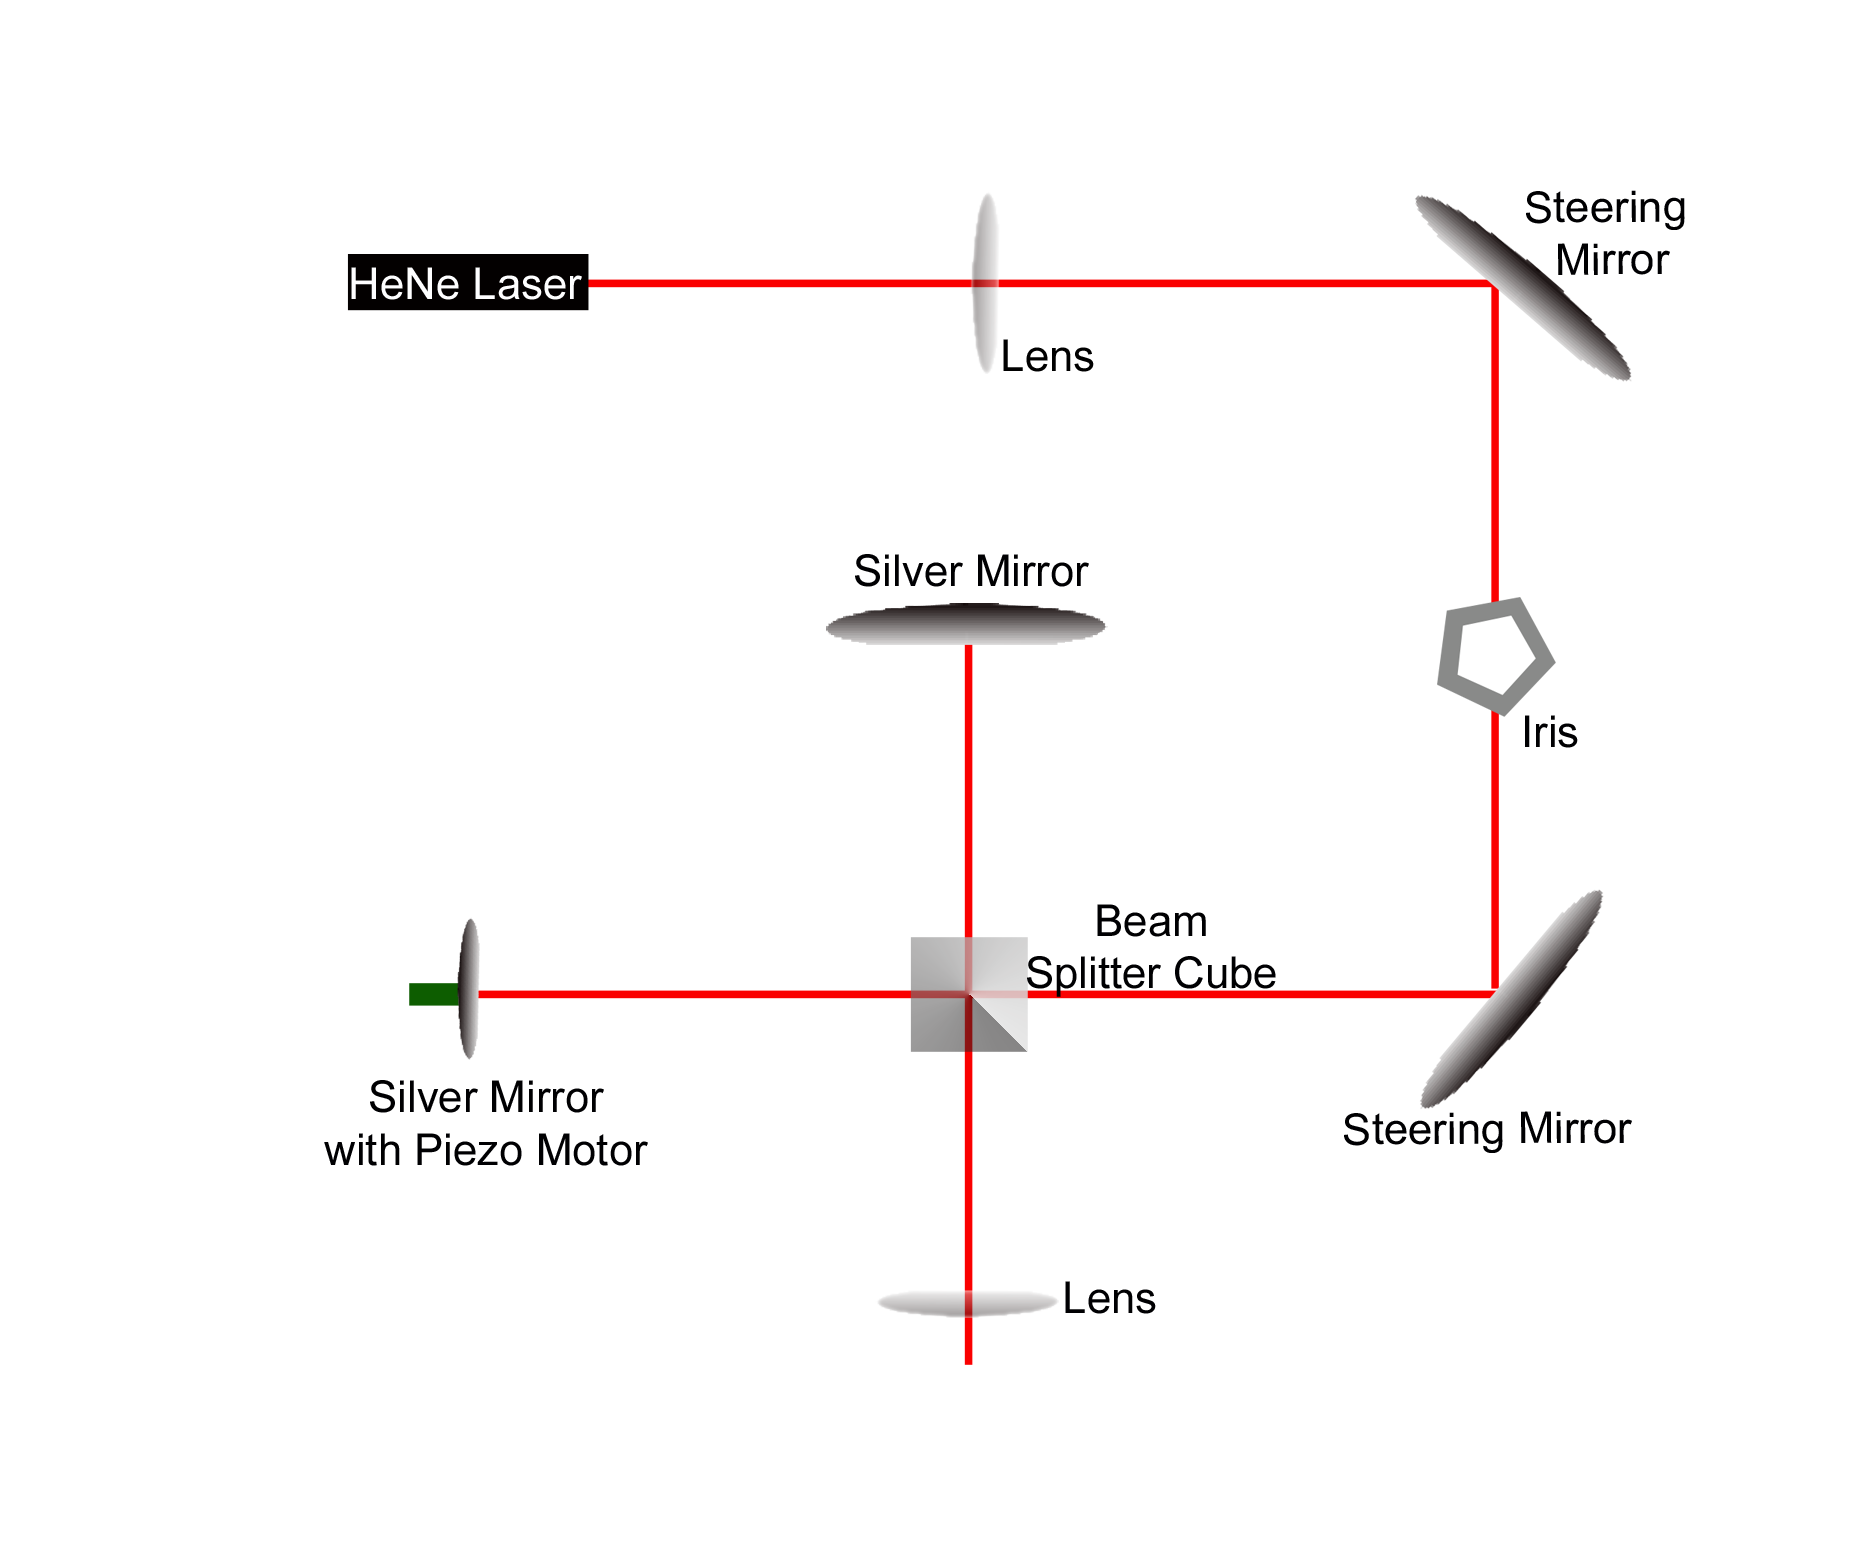
\includegraphics[width=5in]{Interferometer}}
\end{figure}
<<<<<<< HEAD
\newpage
Fig.~\ref{fig:interferometer} Legend:
\begin{enumerate} \itemsep1pt \parskip0pt \parsep0pt
 %  \setcounter[Alph]{1}
   \item[A] He-Ne Laser in ULM-TILT Mount
   \item[B] Lens 1 - 1.0 inch Lens in Kinematic Optics Mount
   \item[C] Mirror 1 - 1.0 inch Silvered Mirror on Kinematic Mirror Mount
   \item[D] Iris
   \item[E] Mirror 2 - 1.0 inch Silvered Mirror on Kinematic Mirror Mount
   \item[F] Beam Splitter Cube on Kinematic Platform Mount
   \item[G] Mirror 3 - 1.0 inch Silvered Mirror on Kinematic Mirror Mount
   \item[H] Piezo Mirror - 0.5 inch Silvered Mirror and Piezo stack on Kinematic Mirror Mount
   \item[I] Photo Diode - DET36A Photo Diode

    \emph{Alternative}: Lens 2 - 1.0 inch Lens in Kinematic Optics Mount
\end{enumerate}
=======
>>>>>>> dbefca72415b5a838a86ae9ff3b0ba994f359908
